\documentclass[11pt,a4paper]{article}

\usepackage[provide=*,spanish]{babel}
\usepackage[utf8]{inputenc}
\usepackage[T1]{fontenc}
\usepackage{lmodern}
\usepackage[margin=2.35cm]{geometry}
\usepackage{amsmath}
\usepackage{amssymb}
\usepackage{booktabs}
\usepackage{longtable}
\usepackage{tabularx}
\usepackage{array}
\usepackage{enumitem}
\usepackage{listings}
\usepackage{xcolor}
\usepackage{microtype}
\usepackage{parskip}
\usepackage{titlesec}
\usepackage{hyperref}
\usepackage{graphicx}
\usepackage{caption}
\usepackage{subcaption}
\usepackage{float}

\definecolor{azulWCD}{RGB}{17,67,112}
\definecolor{azulClaro}{RGB}{232,241,249}
\definecolor{grisCodigo}{RGB}{247,247,247}
\definecolor{verdeCodigo}{RGB}{25,110,55}
\definecolor{rojoCodigo}{RGB}{145,35,35}
\definecolor{tituloColor}{RGB}{0,55,110}
\definecolor{reglaColor}{RGB}{0,90,160}

\hypersetup{
  colorlinks=true,
  linkcolor=azulWCD,
  urlcolor=azulWCD,
  citecolor=azulWCD,
  pdftitle={Efecto del tratamiento termico S(alpha,beta) en el WCD: transporte de neutrones y respuesta electromagnetica},
  pdfauthor={Jaime A. Betancourt}
}

\lstdefinestyle{shstyle}{
  language=bash,
  backgroundcolor=\color{grisCodigo},
  basicstyle=\ttfamily\footnotesize,
  keywordstyle=\color{azulWCD}\bfseries,
  commentstyle=\color{verdeCodigo}\itshape,
  stringstyle=\color{rojoCodigo},
  breaklines=true,
  frame=single,
  rulecolor=\color{gray!40},
  showstringspaces=false,
  columns=fullflexible,
  keepspaces=true
}
\lstset{style=shstyle}

\titleformat{\section}{\normalfont\Large\bfseries\color{azulWCD}}
  {\thesection.}{0.6em}{}
\titleformat{\subsection}{\normalfont\large\bfseries}
  {\thesubsection.}{0.5em}{}
\setlist{itemsep=0.25em,topsep=0.4em}
\renewcommand{\arraystretch}{1.18}
\setlength{\emergencystretch}{2em}

\newcommand{\codigo}[1]{\nolinkurl{#1}}
\newcommand{\archivo}[1]{\path{#1}}
\newcommand{\var}[1]{\texttt{#1}}
\newcommand{\sab}{$S(\alpha,\beta)$}

\begin{document}
\pagestyle{empty}

%------------------------------------------------
% PORTADA
%------------------------------------------------
\begin{titlepage}
\begin{center}

\vspace*{0.5cm}
\textcolor{reglaColor}{\rule{\linewidth}{1.2pt}}

\vspace{1.3cm}
{\Large\scshape Universidad Industrial de Santander}\\[0.2cm]
{\large Escuela de Física --- Facultad de Ciencias}\\[0.2cm]
{\large Doctorado en Física}

\vspace{2.2cm}
{\Huge\bfseries\color{tituloColor} Efecto del tratamiento térmico\\[0.2cm]
S($\alpha,\beta$) en el detector Cherenkov de agua}

\vspace{1.8cm}
{\large\textbf{Barrido en energía de 1\,meV a 1\,keV con dos listas de física:}}\\[0.15cm]
{\large\textbf{transporte de neutrones y respuesta electromagnética del detector}}

\vspace{0.6cm}
\begin{minipage}{0.82\linewidth}
\centering
\textit{``Mismo ejecutable, misma geometría, mismos neutrones: solo cambia cómo se dispersa el hidrógeno ligado del agua''}
\end{minipage}

\vfill

{\large\textbf{Autor}}\\[0.15cm]
Jaime A. Betancourt\\[0.1cm]
Doctorado en Física, Universidad Industrial de Santander

\vspace{1.2cm}
\textcolor{reglaColor}{\rule{0.5\linewidth}{0.6pt}}

\vspace{1cm}
29 de septiembre de 2026

\vspace{1cm}
\textcolor{reglaColor}{\rule{\linewidth}{1.2pt}}

\end{center}
\end{titlepage}

\pagestyle{plain}

\begin{abstract}
Se cuantifica el efecto del tratamiento térmico \sab{} para el hidrógeno ligado en el agua sobre el transporte y la captura de neutrones en el detector Cherenkov de agua (WCD) de la tesis. Con un mismo ejecutable de MEIGA/Geant4, la misma geometría (Sidelnik et~al. 2020b: acero de 0.5\,mm, Tyvek de 0.12\,mm, PMT al 65\,\% de la altura) y agua pura, se simularon 10\,000 neutrones monoenergéticos a 16 energías entre 1\,meV y 1\,keV, con dos físicas: QGSP\_BERT\_HP con \sab{} y QGSP\_BERT\_HP sin \sab{} (hidrógeno como gas libre). El efecto de \sab{} sobre la fracción capturada en el agua \textbf{cambia de signo en $E_0\approx0.34$\,eV}: por debajo la reduce hasta en 8.6 puntos porcentuales (a 25\,meV: $19.70\pm0.40$\,\% frente a $28.31\pm0.45$\,\%) y por encima la aumenta hasta en 8.4 puntos (a 1\,keV: $41.90\pm0.49$\,\% frente a $33.54\pm0.47$\,\%), con significancias de 5 a 14$\sigma$. El análisis de los destinos de los neutrones, de la profundidad y del tiempo de captura identifica el mecanismo: \sab{} acorta la difusión térmica; las capturas ocurren más cerca de la superficie, la vida media térmica efectiva sube de $140.7\pm1.5$ a $161.8\pm1.5\,\mu$s y la tasa de fuga baja en $\approx40$\,\%. Esto aumenta el albedo de la tapa para neutrones que llegan casi térmicos y reduce la fuga para los que se termalizan en profundidad. En consecuencia, el máximo de captura entre 0.3 y 10\,eV descrito con la Campaña~1 es una propiedad del modelo de gas libre: con \sab{} la captura crece de forma monótona y se estabiliza en $\approx42$\,\% por encima de 10\,eV.

La segunda parte sigue la cadena electromagnética hasta la carga del PMT. La eficiencia de detección ($Q\geq1$\,pe) es del 8 al 19\,\% por neutrón incidente y reproduce el efecto de \sab{} ($-34$\,\% a 25\,meV, $+21$\,\% a 1\,keV), con el cruce desplazado a $\approx0.7$\,eV. Sus dos cuellos de botella son geométricos: como las capturas ocurren a pocos centímetros de la superficie, solo el 54--64\,\% de los $\gamma$ de 2.2\,MeV interactúa en el agua, y solo el 1.30\,\% de los fotones Cherenkov creados produce un fotoelectrón. El efecto Compton en el agua representa el 87\,\% de las interacciones $\gamma$ y sus electrones emiten el 94\,\% de la luz, aunque solo el 21\,\% supera el umbral Cherenkov. A energías bajas, las capturas en el acero de la tapa aportan hasta un tercio de los eventos detectados, con una carga media de 9.1\,pe frente a 2.5\,pe de una captura en hidrógeno. Ningún eslabón electromagnético depende de \sab{} salvo a través de la profundidad de captura.
\end{abstract}

\tableofcontents
\newpage

%------------------------------------------------
\section{Motivación}
%------------------------------------------------

La tesis caracteriza el WCD con dos campañas de simulación. La Campaña~1 (febrero de 2025) usó QGSP\_BERT\_HP sin tratamiento térmico: por debajo de 4\,eV el hidrógeno se trata como un núcleo libre con movimiento térmico (modelo de gas libre). La Campaña~2 (septiembre de 2026) incorporó \var{G4ThermalNeutrons}, que sustituye ese modelo por la ley de dispersión \sab{} del hidrógeno ligado en el agua (\var{TS\_H\_of\_Water}). A 25\,meV la Campaña~2 capturaba en el agua unas 0.69 veces lo que la Campaña~1.
%, pero las dos campañas diferían además en la geometría (acero de 0.05 frente a 0.5\,mm, posición del PMT), de modo que no era posible atribuir la diferencia a una sola causa.

Este informe aísla el efecto de \sab{}: ambas físicas se ejecutan con el mismo ejecutable, la misma geometría, el mismo medio y los mismos neutrones incidentes, y se recorre la energía inicial desde neutrones fríos (1\,meV) hasta intermedios (1\,keV), por encima del límite de aplicación de \sab{} (4\,eV).

%------------------------------------------------
\section{Configuración de las simulaciones}
%------------------------------------------------

\subsection{Código y selección de la física}

Todas las corridas usan el ejecutable \var{G4WCDSimulator} de MEIGA compilado con Geant4 10.7.4 (10.07.p04) dentro del contenedor Docker del autor, recompilado el 28 de septiembre de 2026 a partir del código de la rama \var{main} del repositorio \archivo{wcd-nacl-crns-simulations}. La física se elige en el archivo de configuración con la clave \var{Simulation.PhysicsName}:

\begin{table}[H]
\centering
\small
\begin{tabularx}{\linewidth}{lX}
\toprule
\var{PhysicsName} & Física construida por \var{G4MPhysicsList} \\
\midrule
\var{QGSP\_BERT\_HP} & QGSP\_BERT\_HP + \var{G4ThermalNeutrons} (\sab{} para $E<4$\,eV). Física de la Campaña~2. \\
\var{QGSP\_BERT\_HP\_NoThermal} & QGSP\_BERT\_HP sin \var{G4ThermalNeutrons}: hidrógeno como gas libre. Física de la Campaña~1. \\
\bottomrule
\end{tabularx}
\end{table}

Los materiales son idénticos en ambos casos: el agua conserva el elemento \var{TS\_H\_of\_Water}; sin \var{G4ThermalNeutrons} registrado, Geant4 toma para él los datos ordinarios del hidrógeno ($Z=1$) de la biblioteca G4NDL. Durante la preparación de estas pruebas se detectó que \var{G4WCDSimulator} ignoraba \var{PhysicsName} y usaba siempre QGSP\_BERT\_HP; se corrigió para que lea el valor de la configuración (commit \var{0fa4db1}). Las corridas previas de la Campaña~2 no se ven afectadas, porque sus configuraciones pedían precisamente QGSP\_BERT\_HP. Cada corrida verifica en su registro la línea de física registrada (\var{RegisterPhysics: G4ThermalNeutrons} o \var{RegisterPhysics: QGSP\_BERT\_HP without S(alpha,beta)}), y las 32 corridas la superaron.

\subsection{Geometría, medio e inyección}

La geometría se fija en el propio \archivo{DetectorList.xml} de la prueba, para no depender del \archivo{DetectorProperties.xml} de la carpeta de compilación, que CMake sobrescribe al reconfigurar el proyecto. Los valores coinciden con los de Sidelnik et~al. (2020b) y con los medidos en los datos de la Campaña~2:

\begin{table}[H]
\centering
\small
\begin{tabularx}{\linewidth}{lX}
\toprule
Parámetro & Valor \\
\midrule
Volumen activo & cilindro de agua pura de 48\,cm de radio y 133\,cm de altura \\
Revestimiento & Tyvek de 0.12\,mm \\
Tanque & acero inoxidable de 0.5\,mm (tapa, pared y fondo) \\
PMT & sobre el eje, cara plana a 86.5\,cm del fondo (65\,\% de la altura) \\
Superficie del agua & $z = 133.062$\,cm \\
Inyección & vertical hacia abajo desde $z=200$\,cm, uniforme en un círculo de 40\,cm de radio \\
Neutrones por corrida & 10\,000 \\
Energías $E_0$ & 1, 2.5, 5, 7, 10, 25, 50, 80, 100, 300, 500, 700\,meV; 1, 10, 100\,eV; 1\,keV \\
%Modo de simulación & \var{eFast} (no afecta al transporte de neutrones) \\
\bottomrule
\end{tabularx}
\end{table}

Las 16 energías reproducen la malla de la Campaña~1 original hasta 1\,keV. El momento del neutrón se calcula como $p=\sqrt{E^2+2mE}$; para 25\,meV se obtiene $6.85407\times10^{-6}$\,GeV/$c$, idéntico al archivo de flujo de la Campaña~2. Cada corrida verifica la energía inyectada en \archivo{neutrones-incidentes.tsv}.

\subsection{Magnitudes analizadas}

Para cada neutrón primario se clasifica su destino con el archivo \archivo{pasos-neutrones.tsv}:
\begin{itemize}
  \item \textbf{captura en el agua}: el último paso es \var{nCapture} en el agua;
  \item \textbf{captura en la estructura}: \var{nCapture} en el acero o el Tyvek;
  \item \textbf{reflexión por la tapa}, \textbf{escape lateral} o \textbf{transmisión por el fondo}: la cara de salida se toma del último paso dentro de un material del tanque (no de la posición final en el borde del mundo); las capturas y reacciones $(n,p)$ en el aire posteriores a la salida cuentan como escape por esa cara;
  \item \textbf{desviado en el aire}: el neutrón se dispersa en los 67\,cm de aire entre la fuente y la tapa y nunca entra en el tanque.
\end{itemize}
Para las capturas en el agua se registran además el número de dispersiones elásticas previas $N$, la profundidad bajo la superficie del agua, el tiempo transcurrido desde que el neutrón toca la tapa (se descuenta el vuelo por el aire) y la energía cinética al comenzar el paso de captura. Las incertidumbres de las fracciones son binomiales ($1\sigma$).

%------------------------------------------------
\section{Validación}
%------------------------------------------------

\begin{itemize}
  \item \textbf{Selección de física.} Las 32 corridas registran la física pedida. Con la misma geometría, las dos físicas difieren en 5 a 14$\sigma$ en casi todas las energías, lo que descarta que el cambio de física no se aplique.
  \item \textbf{Reproducción de la Campaña~2.} A 25\,meV con \sab{}, una prueba de 10\,000 neutrones dio $18.70\pm0.39$\,\% de captura en el agua y $\langle N\rangle=88.7$, frente a $19.62\pm0.13$\,\% y 90.4 en la Campaña~2 (100\,000 neutrones). $\langle N\rangle$ coincide; la captura difiere en 2.2$\sigma$. La corrida de agua pura de la Campaña~2 (14-09-2026) se hizo con el ejecutable anterior a la recompilación del 15-09-2026, por lo que no puede excluirse una pequeña diferencia de código.
  \item \textbf{Reproducción de la Campaña~1.} La física sin \sab{} reproduce el $\langle N\rangle$ de los datos originales de febrero de 2025: 53.3 frente a 52.2 a 25\,meV y 61.3 frente a 60.4 a 1\,eV.
  \item \textbf{Estabilidad estadística.} El punto de 1\,eV sin \sab{} se simuló dos veces: $32.84\pm0.47$\,\% y $34.49\pm0.48$\,\% (2.5$\sigma$). Con 10\,000 neutrones, fluctuaciones de este tamaño aparecen ocasionalmente; no afectan a las conclusiones cualitativas, pero las cifras definitivas deben obtenerse con más estadística (sección~\ref{sec:limitaciones}).
  %\item \textbf{Integridad de los datos.} El archivo transferido desde el contenedor (1.6\,GB comprimido) pasó la verificación de \var{gzip}; la tabla recalculada a partir de los TSV transferidos es idéntica a la calculada en el contenedor, y en cada corrida la suma de las seis categorías de destino es igual al número de neutrones incidentes.
\end{itemize}

%------------------------------------------------
\section{Resultados}
%------------------------------------------------

\subsection{Captura en el agua y número de colisiones}

\begin{figure}[H]
\centering
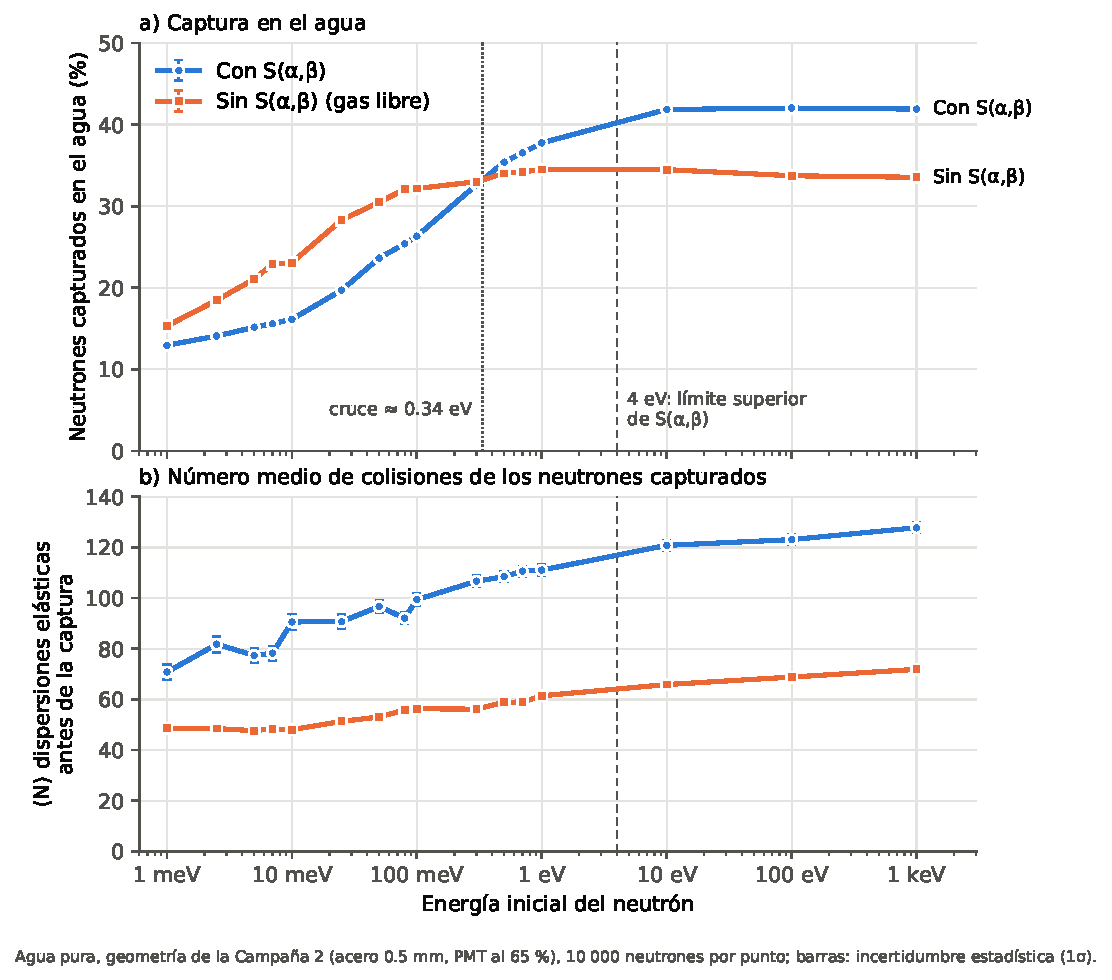
\includegraphics[width=0.86\linewidth]{figuras/fig_captura_N_vs_energia.pdf}
\caption{(a) Fracción de neutrones incidentes capturados en el agua y (b) número medio de dispersiones elásticas antes de la captura, con y sin \sab{}. Línea discontinua: 4\,eV, límite superior de \sab{}; línea punteada: energía de cruce.}
\label{fig:captura}
\end{figure}

\begin{table}[H]
\centering
\small
\begin{tabular}{lrrrrrr}
\toprule
& \multicolumn{2}{c}{Captura en el agua (\%)} & & & \multicolumn{2}{c}{$\langle N\rangle$} \\
\cmidrule(lr){2-3}\cmidrule(lr){6-7}
$E_0$ & con $S(\alpha,\beta)$ & sin $S(\alpha,\beta)$ & Efecto (pts) & Signif. & con & sin \\
\midrule
1\,meV & $12.95\pm0.34$ & $15.32\pm0.36$ & $-2.37$ & $-4.8\sigma$ & $70.8$ & $48.7$ \\
2.5\,meV & $14.09\pm0.35$ & $18.47\pm0.39$ & $-4.38$ & $-8.4\sigma$ & $81.8$ & $48.5$ \\
5\,meV & $15.16\pm0.36$ & $21.07\pm0.41$ & $-5.91$ & $-10.8\sigma$ & $77.4$ & $47.7$ \\
7\,meV & $15.61\pm0.36$ & $22.90\pm0.42$ & $-7.29$ & $-13.2\sigma$ & $78.2$ & $48.4$ \\
10\,meV & $16.14\pm0.37$ & $23.08\pm0.42$ & $-6.94$ & $-12.4\sigma$ & $90.6$ & $48.1$ \\
25\,meV & $19.70\pm0.40$ & $28.31\pm0.45$ & $-8.61$ & $-14.3\sigma$ & $90.7$ & $51.4$ \\
50\,meV & $23.64\pm0.42$ & $30.48\pm0.46$ & $-6.84$ & $-11.0\sigma$ & $96.7$ & $53.1$ \\
80\,meV & $25.40\pm0.44$ & $32.07\pm0.47$ & $-6.67$ & $-10.4\sigma$ & $92.1$ & $55.9$ \\
100\,meV & $26.32\pm0.44$ & $32.16\pm0.47$ & $-5.84$ & $-9.1\sigma$ & $99.4$ & $56.3$ \\
300\,meV & $32.62\pm0.47$ & $33.00\pm0.47$ & $-0.38$ & $-0.6\sigma$ & $106.7$ & $56.2$ \\
500\,meV & $35.39\pm0.48$ & $34.02\pm0.47$ & $+1.37$ & $+2.0\sigma$ & $108.5$ & $58.9$ \\
700\,meV & $36.54\pm0.48$ & $34.20\pm0.47$ & $+2.34$ & $+3.5\sigma$ & $110.6$ & $59.0$ \\
1\,eV & $37.76\pm0.48$ & $34.49\pm0.48$ & $+3.27$ & $+4.8\sigma$ & $111.0$ & $61.4$ \\
10\,eV & $41.85\pm0.49$ & $34.48\pm0.48$ & $+7.37$ & $+10.7\sigma$ & $120.8$ & $65.9$ \\
100\,eV & $42.03\pm0.49$ & $33.73\pm0.47$ & $+8.30$ & $+12.2\sigma$ & $123.1$ & $68.8$ \\
1\,keV & $41.90\pm0.49$ & $33.54\pm0.47$ & $+8.36$ & $+12.3\sigma$ & $127.8$ & $71.9$ \\
\bottomrule
\end{tabular}

\caption{Captura en el agua (porcentaje de los 10\,000 neutrones incidentes) y $\langle N\rangle$ de los neutrones capturados. ``Efecto'' es la diferencia con menos sin \sab{}, en puntos porcentuales, y ``Signif.'' su cociente con la incertidumbre combinada.}
\label{tab:captura}
\end{table}

Los resultados principales son:
\begin{itemize}
  \item \textbf{El efecto de \sab{} cambia de signo en $E_0\approx0.34$\,eV} (interpolación logarítmica entre 0.3 y 0.5\,eV). Por debajo, \sab{} reduce la captura; el efecto es máximo entre 7 y 25\,meV ($-7$ a $-8.6$ puntos). Por encima, la aumenta y se estabiliza en $\approx+8$ puntos desde 10\,eV.
  \item \textbf{El efecto persiste por encima de 4\,eV}, donde \sab{} no actúa sobre el neutrón incidente: todo neutrón termina su historia difundiéndose térmicamente en el agua, y es en esa fase donde interviene \sab{}.
  \item \textbf{La forma de la curva cambia.} Sin \sab{} la captura presenta un máximo amplio de $\approx34.5$\,\% entre 0.7 y 10\,eV y decrece ligeramente hasta 1\,keV. Con \sab{} crece de forma monótona desde el 13\,\% a 1\,meV y se estabiliza en $\approx42$\,\% por encima de 10\,eV.
  \item \textbf{$\langle N\rangle$ es entre 1.4 y 1.8 veces mayor con \sab{}} en todo el rango: el hidrógeno ligado dispersa más en energías térmicas, y la razón entre dispersión y absorción aumenta.
\end{itemize}

\subsection{Destinos de los neutrones}

\begin{figure}[H]
\centering
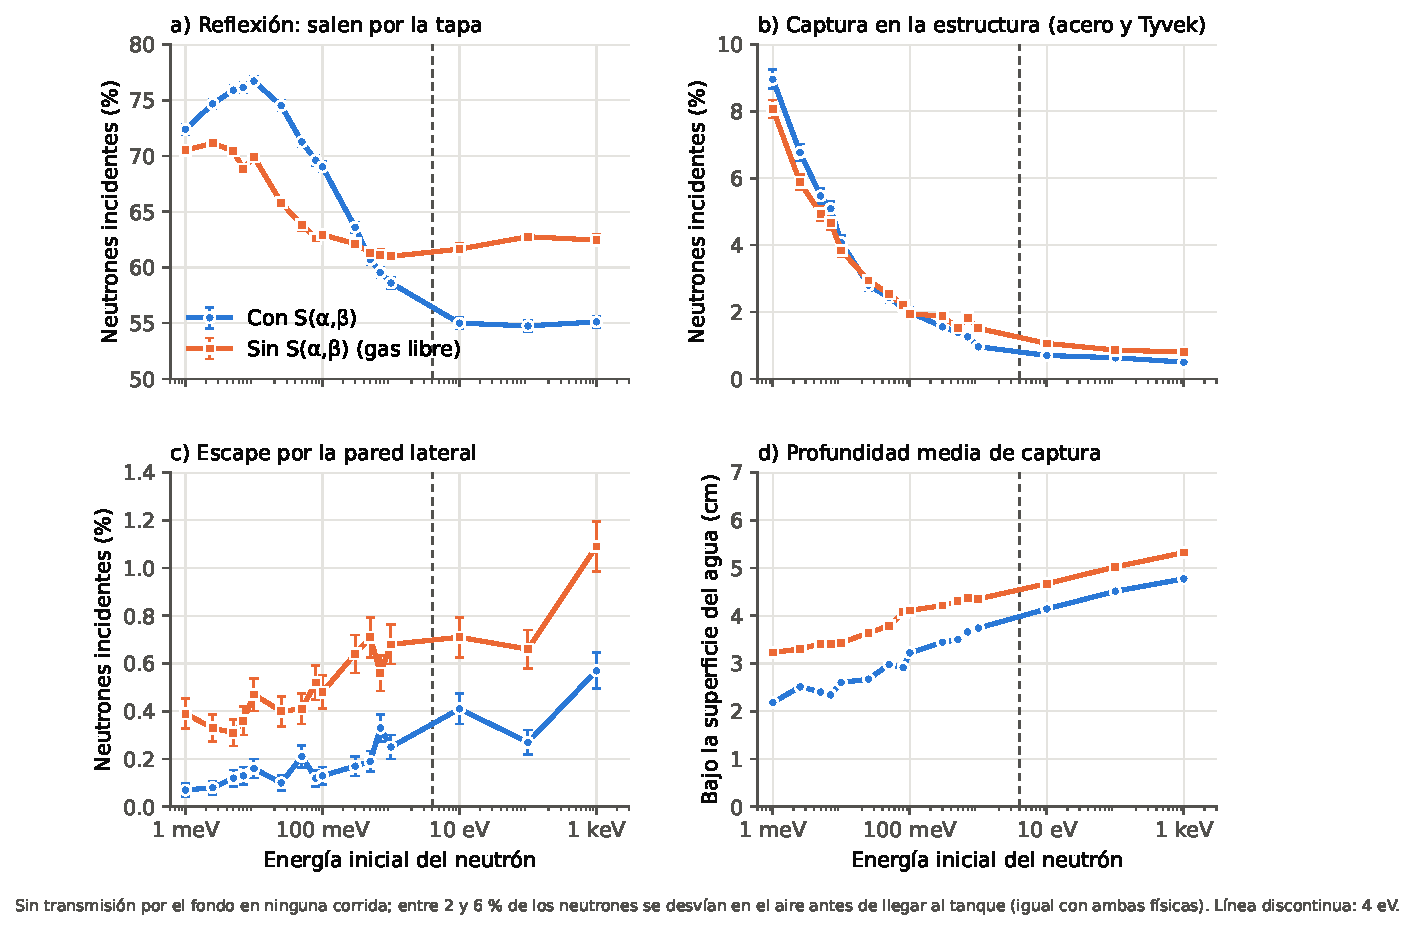
\includegraphics[width=\linewidth]{figuras/fig_destinos_vs_energia.pdf}
\caption{Destinos de los neutrones incidentes: (a) reflexión por la tapa, (b) captura en la estructura, (c) escape lateral y (d) profundidad media de captura bajo la superficie del agua.}
\label{fig:destinos}
\end{figure}

\begin{itemize}
  \item \textbf{La reflexión por la tapa es el destino dominante}: entre el 55 y el 77\,\% de los neutrones incidentes. Es la imagen especular de la captura: con \sab{} la reflexión es mayor por debajo de 0.34\,eV (máximo de 76.7\,\% a 10\,meV frente a 70\,\%) y menor por encima (55\,\% frente a 62\,\% desde 10\,eV).
  \item \textbf{La captura en la estructura} decrece del 9\,\% a 1\,meV al 0.5\,\% a 1\,keV, siguiendo la ley $1/v$ del hierro, y es casi igual con ambas físicas.
  \item \textbf{El escape lateral} es inferior al 1.2\,\% y menor con \sab{}. \textbf{No hay transmisión por el fondo} en ninguna corrida: 133\,cm de agua absorben o devuelven todo neutrón.
  \item \textbf{Entre el 2 y el 6\,\%} de los neutrones se desvían en el aire antes de llegar al tanque; la fracción es la misma con ambas físicas, como corresponde a que \sab{} no actúa en el aire.
\end{itemize}

La tabla completa de destinos se incluye en el apéndice~\ref{app:destinos}.

\subsection{Profundidad de captura}

\begin{figure}[H]
\centering
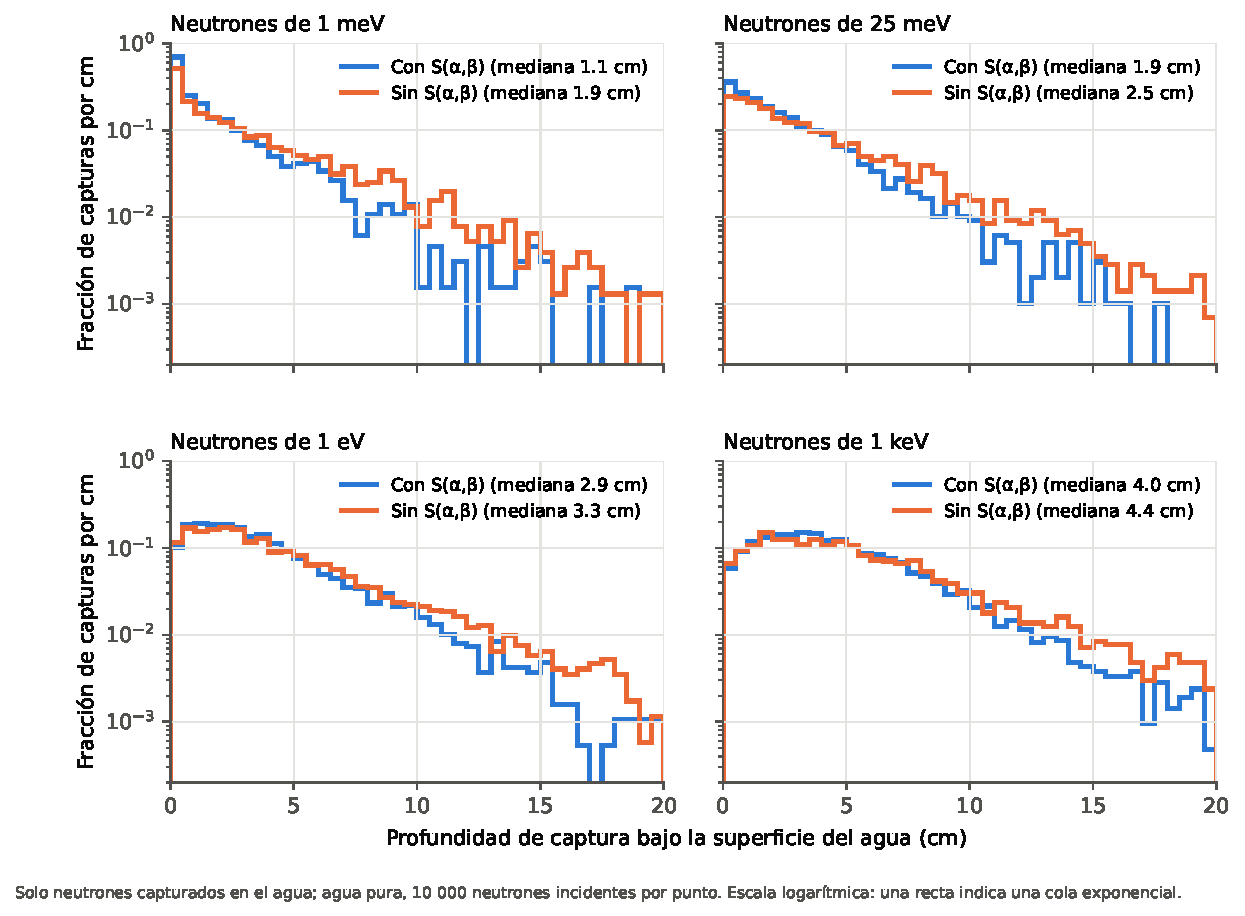
\includegraphics[width=\linewidth]{figuras/fig_profundidad_captura.pdf}
\caption{Distribución de la profundidad de captura bajo la superficie del agua para cuatro energías iniciales. Escala logarítmica: una recta corresponde a una cola exponencial.}
\label{fig:profundidad}
\end{figure}

Casi todas las capturas ocurren en los primeros 10\,cm bajo la superficie del agua: la mediana va de 1.1\,cm (1\,meV, con \sab{}) a 4.4\,cm (1\,keV, sin \sab{}). Para neutrones fríos y térmicos la distribución es máxima en la superficie y decae exponencialmente; para neutrones de 1\,eV y 1\,keV primero crece hasta 2--4\,cm, donde el neutrón termina de frenarse, y después decae. \textbf{Con \sab{} las capturas ocurren más cerca de la superficie en todas las energías}, y la cola exponencial decae más rápido, lo que indica una longitud de difusión térmica más corta.

\subsection{Tiempo, vida media térmica y energía de captura}

\begin{figure}[H]
\centering
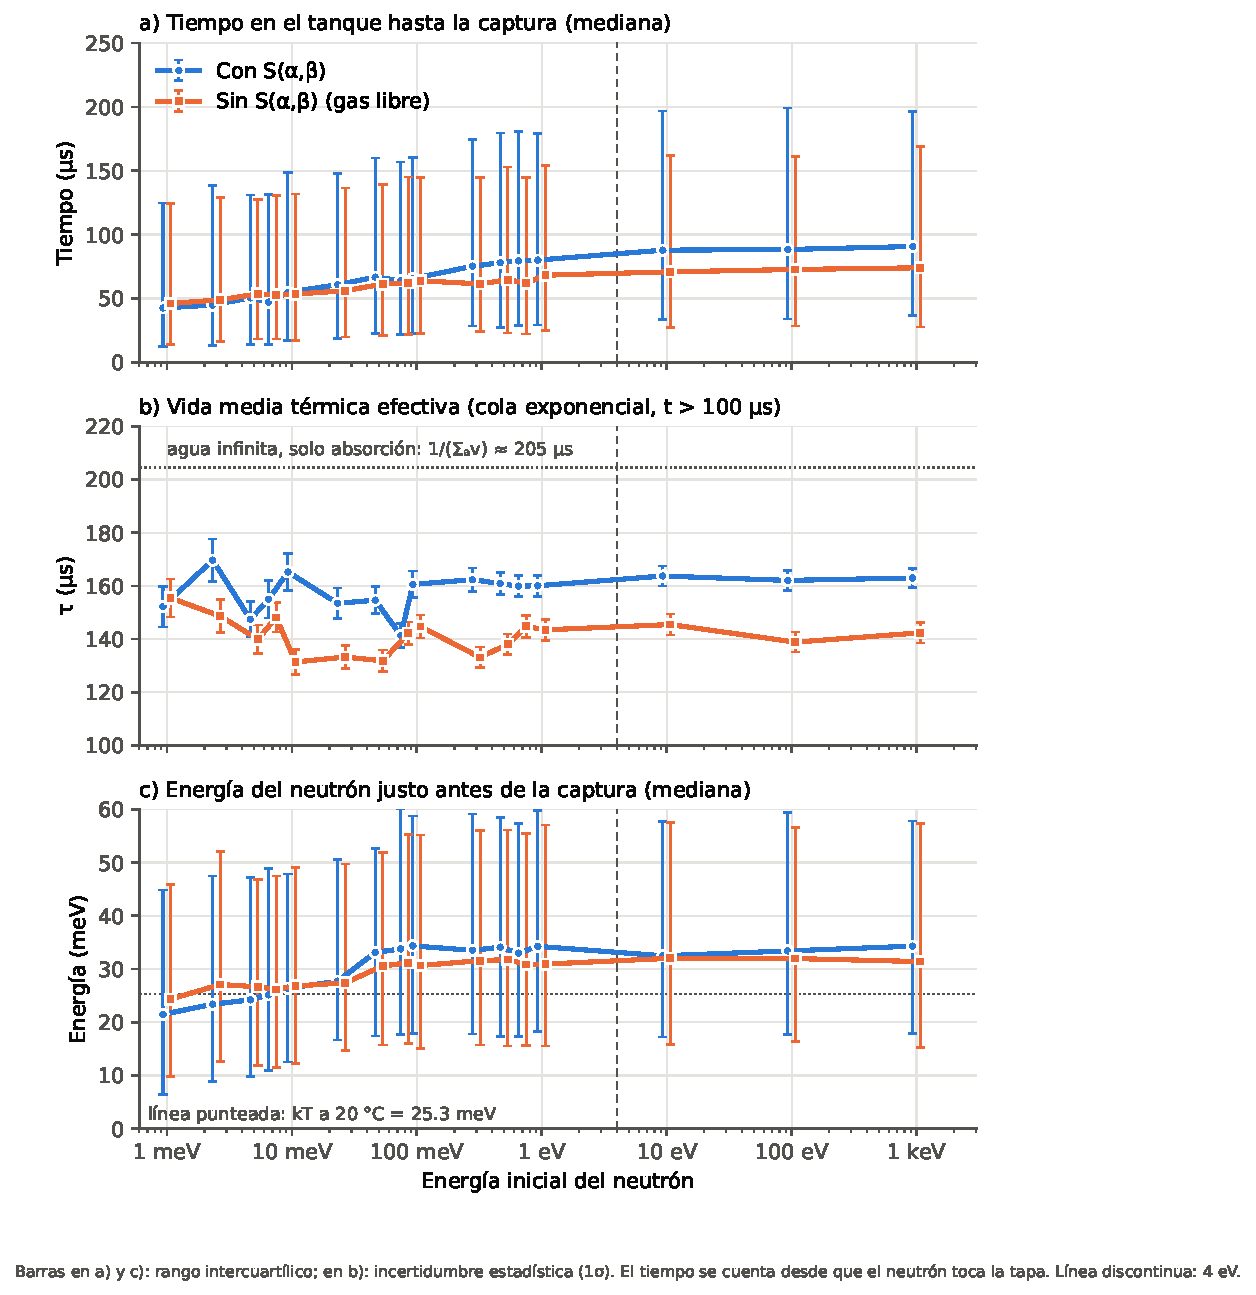
\includegraphics[width=0.86\linewidth]{figuras/fig_tiempo_energia_captura.pdf}
\caption{(a) Tiempo en el tanque hasta la captura (mediana y rango intercuartílico), (b) vida media térmica efectiva estimada con la cola exponencial ($t>100\,\mu$s) y (c) energía del neutrón al comenzar el paso de captura.}
\label{fig:tiempo}
\end{figure}

\begin{table}[H]
\centering
\small
\begin{tabular}{lrrrrrrrr}
\toprule
& \multicolumn{2}{c}{Prof. mediana (cm)} & \multicolumn{2}{c}{$t$ mediano ($\mu$s)} & \multicolumn{2}{c}{$\tau_\mathrm{ef}$ ($\mu$s)} & \multicolumn{2}{c}{$E$ mediana (meV)} \\
\cmidrule(lr){2-3}\cmidrule(lr){4-5}\cmidrule(lr){6-7}\cmidrule(lr){8-9}
$E_0$ & con & sin & con & sin & con & sin & con & sin \\
\midrule
1\,meV & 1.1 & 1.9 & 43 & 46 & $152\pm8$ & $155\pm7$ & 21.5 & 24.3 \\
2.5\,meV & 1.4 & 2.1 & 45 & 49 & $170\pm8$ & $149\pm6$ & 23.4 & 27.1 \\
5\,meV & 1.5 & 2.2 & 51 & 54 & $147\pm7$ & $140\pm5$ & 24.2 & 26.7 \\
7\,meV & 1.4 & 2.2 & 47 & 53 & $155\pm7$ & $148\pm6$ & 25.2 & 26.2 \\
10\,meV & 1.6 & 2.4 & 55 & 53 & $165\pm7$ & $131\pm5$ & 26.4 & 26.8 \\
25\,meV & 1.9 & 2.5 & 61 & 56 & $153\pm6$ & $133\pm4$ & 27.7 & 27.4 \\
50\,meV & 2.1 & 2.8 & 67 & 61 & $155\pm5$ & $132\pm4$ & 33.1 & 30.6 \\
80\,meV & 2.1 & 3.0 & 64 & 62 & $141\pm5$ & $142\pm4$ & 33.8 & 31.2 \\
100\,meV & 2.3 & 3.0 & 66 & 64 & $161\pm5$ & $145\pm4$ & 34.4 & 30.7 \\
300\,meV & 2.7 & 3.1 & 75 & 61 & $162\pm4$ & $133\pm4$ & 33.5 & 31.6 \\
500\,meV & 2.7 & 3.3 & 78 & 65 & $161\pm4$ & $138\pm4$ & 34.1 & 31.8 \\
700\,meV & 2.9 & 3.2 & 80 & 62 & $160\pm4$ & $145\pm4$ & 33.0 & 30.8 \\
1\,eV & 2.9 & 3.3 & 80 & 68 & $160\pm4$ & $143\pm4$ & 34.3 & 30.9 \\
10\,eV & 3.5 & 3.6 & 88 & 71 & $164\pm4$ & $145\pm4$ & 32.5 & 32.0 \\
100\,eV & 3.9 & 4.1 & 88 & 73 & $162\pm4$ & $139\pm4$ & 33.4 & 32.0 \\
1\,keV & 4.0 & 4.4 & 91 & 74 & $163\pm4$ & $142\pm4$ & 34.3 & 31.4 \\
\bottomrule
\end{tabular}

\caption{Profundidad mediana de captura, tiempo mediano en el tanque, vida media térmica efectiva $\tau_\mathrm{ef}$ y energía mediana antes de la captura, con y sin \sab{}.}
\label{tab:capturas}
\end{table}

\begin{itemize}
  \item \textbf{Tiempo en el tanque.} La mediana va de 43 a 91\,$\mu$s. Por encima de $\approx0.1$\,eV es mayor con \sab{} (por ejemplo, 91 frente a 74\,$\mu$s a 1\,keV).
  \item \textbf{Vida media térmica efectiva.} Combinando las energías $E_0\geq0.3$\,eV, donde $\tau_\mathrm{ef}$ es estable, se obtiene
  \begin{equation*}
    \tau_\mathrm{ef}^{\,\mathrm{con}} = 161.8\pm1.5\,\mu\mathrm{s},\qquad
    \tau_\mathrm{ef}^{\,\mathrm{sin}} = 140.7\pm1.5\,\mu\mathrm{s}.
  \end{equation*}
  Ambas son menores que la vida media de absorción en agua infinita, $\tau_a=1/(\Sigma_a v)\approx204.5\,\mu$s ($\Sigma_a=0.02223$\,cm$^{-1}$ a 2200\,m/s).
  \item \textbf{Energía de captura.} La mediana de la energía antes de la captura está entre 21 y 34\,meV para todas las energías iniciales, y como mucho el 2\,\% de las capturas ocurre por encima de 0.5\,eV: \textbf{prácticamente toda captura es térmica}. La energía inicial determina dónde se termaliza el neutrón, no cómo se captura.
\end{itemize}

%------------------------------------------------
\section{Interpretación física}
%------------------------------------------------

\subsection{Fuga térmica}

La captura en hidrógeno sigue la ley $1/v$, de modo que el producto $\Sigma_a v$ y, con él, el tiempo de absorción $\tau_a$ no dependen de la forma del espectro térmico. Si la población térmica decae por absorción y por fuga,
\begin{equation}
  \frac{1}{\tau_\mathrm{ef}} = \frac{1}{\tau_a} + \lambda_\mathrm{fuga},
\end{equation}
la diferencia entre las dos vidas medias efectivas se debe únicamente a la fuga:
\begin{equation*}
  \lambda_\mathrm{fuga}^{\,\mathrm{con}} \approx 1.29\times10^{-3}\,\mu\mathrm{s}^{-1},\qquad
  \lambda_\mathrm{fuga}^{\,\mathrm{sin}} \approx 2.22\times10^{-3}\,\mu\mathrm{s}^{-1},
\end{equation*}
es decir, \textbf{con \sab{} la tasa de fuga térmica es $\approx40$\,\% menor}. Es la consecuencia esperada de una sección eficaz de dispersión mayor: el coeficiente de difusión $D=1/(3\Sigma_\mathrm{tr})$ disminuye, y con él la longitud de difusión $L=\sqrt{D/\Sigma_a}$. Las Figuras~\ref{fig:destinos}(d) y~\ref{fig:profundidad} muestran directamente la difusión más corta.

\subsection{Albedo y cambio de signo}

El mismo acortamiento de la difusión produce efectos opuestos según dónde se termalice el neutrón:
\begin{itemize}
  \item \textbf{Neutrones que llegan casi térmicos} ($E_0\lesssim0.34$\,eV). Comienzan a difundirse en la superficie de entrada. En teoría de difusión, el albedo de un medio semiinfinito es
  \begin{equation}
    \beta = \frac{1-2\sqrt{D\,\Sigma_a}}{1+2\sqrt{D\,\Sigma_a}},
  \end{equation}
  que crece cuando $D$ disminuye. Con \sab{} la tapa refleja más y la captura disminuye (Figura~\ref{fig:destinos}a).
  \item \textbf{Neutrones que se termalizan en profundidad} ($E_0\gtrsim0.34$\,eV). Al terminar el frenado se encuentran a varios centímetros de la superficie; con una difusión más corta les resulta más difícil regresar a ella, de modo que la reflexión disminuye y la captura aumenta. Por encima de 10\,eV la profundidad de termalización cambia poco con $E_0$ y el efecto se estabiliza.
\end{itemize}

Los cuatro análisis (captura, destinos, profundidad y tiempo) son consistentes con este mecanismo y no requieren ningún otro.

%------------------------------------------------
\section{Respuesta electromagnética del detector}
\label{sec:em}
%------------------------------------------------

Las secciones anteriores describen el destino de los neutrones. Esta sección sigue la cadena completa que convierte una captura en una señal: los fotones $\gamma$ de la captura, sus interacciones, los electrones secundarios, la luz Cherenkov y la carga del PMT. Se usan los mismos 32 conjuntos de datos.

\subsection{Método}

\begin{itemize}
  \item \textbf{Carga.} El PMT escribe en \archivo{Carga-total.txt} una línea por evento (un neutrón incidente) con el número de fotoelectrones. La línea $i$ corresponde al neutrón con \var{run\_id}~$=i$. La asignación se verificó: los neutrones reflejados por la tapa producen señal en el 0.0\,\% de los casos, y nunca hay carga en un evento sin fotones Cherenkov.
  \item \textbf{Fotones $\gamma$ de captura.} Son las trazas de \archivo{pasos-gamma.tsv} con \var{parent\_id}~$=1$ y \var{creator\_process}~$=$~\var{nCapture}. En \archivo{secundarias-captura-neutron.tsv} el número de traza del secundario aún no está asignado (vale 0), por lo que no sirve para enlazarlos. Un $\gamma$ ``interactúa en el agua'' si tiene al menos un paso Compton, fotoeléctrico o de pares en el agua; la energía transferida es la suma de sus pérdidas en esos pasos. Un $\gamma$ ``se absorbe'' si su última interacción es fotoeléctrica o de pares; si no, sale del tanque, y la cara de salida se determina como para los neutrones.
  \item \textbf{Electrones y luz.} Para cada electrón o positrón se registra el proceso que lo creó, el material y su energía cinética inicial. Cada fotón Cherenkov de \archivo{fotones-cherenkov.tsv} se asigna a su emisor mediante (\var{run\_id}, \var{parent\_track\_id}); los 10.2 millones de fotones quedaron asignados. Los fotones se registran al crearse; en el modo \var{eFast} la eficiencia cuántica se aplica en ese momento, lo que estadísticamente equivale a aplicarla en el PMT.
\end{itemize}

\subsection{Eficiencia de detección}

\begin{figure}[H]
\centering
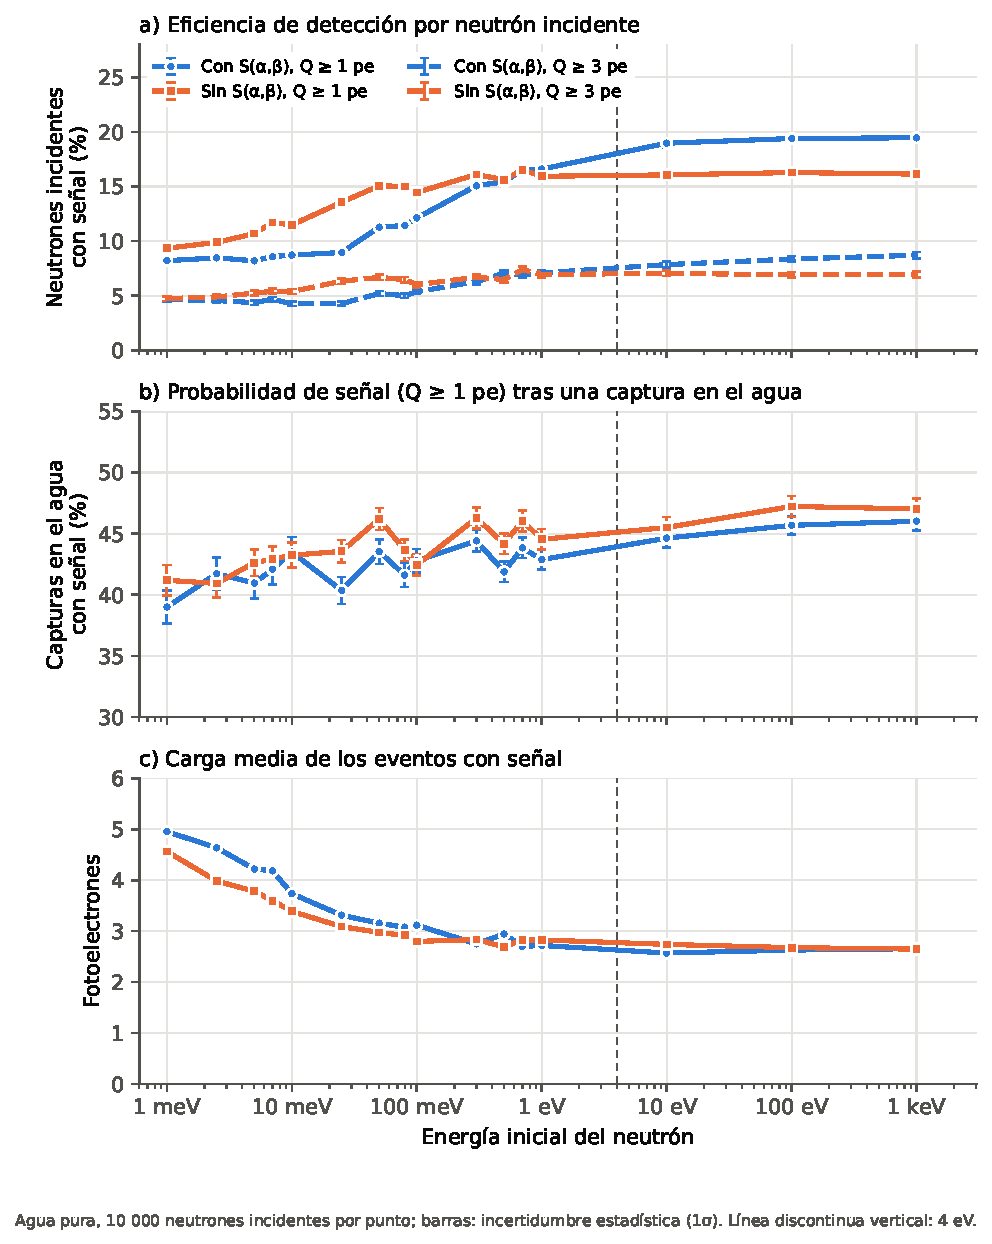
\includegraphics[width=0.84\linewidth]{figuras/fig_eficiencia_deteccion.pdf}
\caption{(a) Fracción de neutrones incidentes que producen al menos 1 y al menos 3 fotoelectrones, (b) probabilidad de señal ($Q\geq1$) una vez capturado el neutrón en el agua y (c) carga media de los eventos con señal.}
\label{fig:eficiencia}
\end{figure}

\begin{table}[H]
\centering
\footnotesize
\begin{tabular}{lrrrrrrrr}
\toprule
& \multicolumn{2}{c}{$\varepsilon$, $Q\geq1$ (\%)} & \multicolumn{2}{c}{$\varepsilon$, $Q\geq3$ (\%)} & \multicolumn{2}{c}{Señal tras captura (\%)} & \multicolumn{2}{c}{$\gamma$ que interactúan (\%)} \\
\cmidrule(lr){2-3}\cmidrule(lr){4-5}\cmidrule(lr){6-7}\cmidrule(lr){8-9}
$E_0$ & con & sin & con & sin & con & sin & con & sin \\
\midrule
1\,meV & $8.20\pm0.27$ & $9.34\pm0.29$ & 4.65 & 4.73 & 39.0 & 41.2 & 54.5 & 56.1 \\
2.5\,meV & $8.46\pm0.28$ & $9.88\pm0.30$ & 4.55 & 4.88 & 41.7 & 40.9 & 55.6 & 56.8 \\
5\,meV & $8.19\pm0.27$ & $10.68\pm0.31$ & 4.36 & 5.23 & 41.0 & 42.6 & 53.5 & 58.3 \\
7\,meV & $8.58\pm0.28$ & $11.69\pm0.32$ & 4.67 & 5.40 & 42.1 & 42.9 & 55.0 & 58.4 \\
10\,meV & $8.71\pm0.28$ & $11.48\pm0.32$ & 4.25 & 5.38 & 43.5 & 43.2 & 56.1 & 58.4 \\
25\,meV & $8.95\pm0.29$ & $13.55\pm0.34$ & 4.27 & 6.32 & 40.4 & 43.5 & 55.5 & 57.9 \\
50\,meV & $11.27\pm0.32$ & $15.07\pm0.36$ & 5.19 & 6.67 & 43.5 & 46.2 & 56.5 & 61.1 \\
80\,meV & $11.43\pm0.32$ & $14.99\pm0.36$ & 5.00 & 6.47 & 41.6 & 43.6 & 56.1 & 58.8 \\
100\,meV & $12.12\pm0.33$ & $14.45\pm0.35$ & 5.36 & 6.00 & 42.8 & 42.4 & 57.8 & 58.7 \\
300\,meV & $15.07\pm0.36$ & $16.10\pm0.37$ & 6.29 & 6.69 & 44.4 & 46.3 & 58.5 & 61.8 \\
500\,meV & $15.42\pm0.36$ & $15.60\pm0.36$ & 7.05 & 6.47 & 41.9 & 44.2 & 56.9 & 60.0 \\
700\,meV & $16.51\pm0.37$ & $16.52\pm0.37$ & 6.86 & 7.38 & 43.8 & 46.0 & 59.8 & 61.5 \\
1\,eV & $16.59\pm0.37$ & $15.93\pm0.37$ & 7.08 & 6.94 & 42.9 & 44.5 & 58.3 & 60.5 \\
10\,eV & $18.96\pm0.39$ & $16.06\pm0.37$ & 7.84 & 7.04 & 44.6 & 45.5 & 60.6 & 61.9 \\
100\,eV & $19.39\pm0.40$ & $16.27\pm0.37$ & 8.35 & 6.91 & 45.7 & 47.2 & 61.3 & 63.3 \\
1\,keV & $19.46\pm0.40$ & $16.13\pm0.37$ & 8.70 & 6.94 & 46.0 & 47.0 & 62.1 & 64.0 \\
\bottomrule
\end{tabular}

\caption{Eficiencia de detección $\varepsilon$ por neutrón incidente para dos umbrales de carga, probabilidad de señal tras una captura en el agua y fracción de los $\gamma$ de 2.2\,MeV que interactúan en el agua, con y sin \sab{}.}
\label{tab:eficiencia}
\end{table}

\begin{itemize}
  \item \textbf{La eficiencia de detección va del 8 al 19\,\%} por neutrón incidente ($Q\geq1$\,pe). Sigue a la captura: con \sab{} es un 34\,\% menor a 25\,meV ($8.95\pm0.29$ frente a $13.55\pm0.34$\,\%) y un 21\,\% mayor a 1\,keV ($19.46\pm0.40$ frente a $16.13\pm0.37$\,\%).
  \item \textbf{El cruce de la eficiencia ocurre hacia 0.7\,eV}, por encima del cruce de la captura (0.34\,eV). Una vez capturado el neutrón en el agua, la probabilidad de señal es del 39--47\,\% y resulta 1--3 puntos menor con \sab{}, porque las capturas son más superficiales y se escapan más $\gamma$.
  \item \textbf{La carga media de los eventos detectados} es mayor a energías bajas (5.0\,pe a 1\,meV frente a 2.6\,pe por encima de 1\,eV). La causa son las capturas en el acero de la tapa: sus $\gamma$ de 7--9\,MeV producen en promedio 9.1\,pe, frente a 2.5\,pe de una captura en hidrógeno, y a 1\,meV constituyen el 38\,\% (con \sab{}) y el 32\,\% (sin \sab{}) de los eventos detectados; por encima de 1\,eV son menos del 3\,\%.
\end{itemize}

\subsection{Contención de los fotones $\gamma$ de 2.2\,MeV}

\begin{figure}[H]
\centering
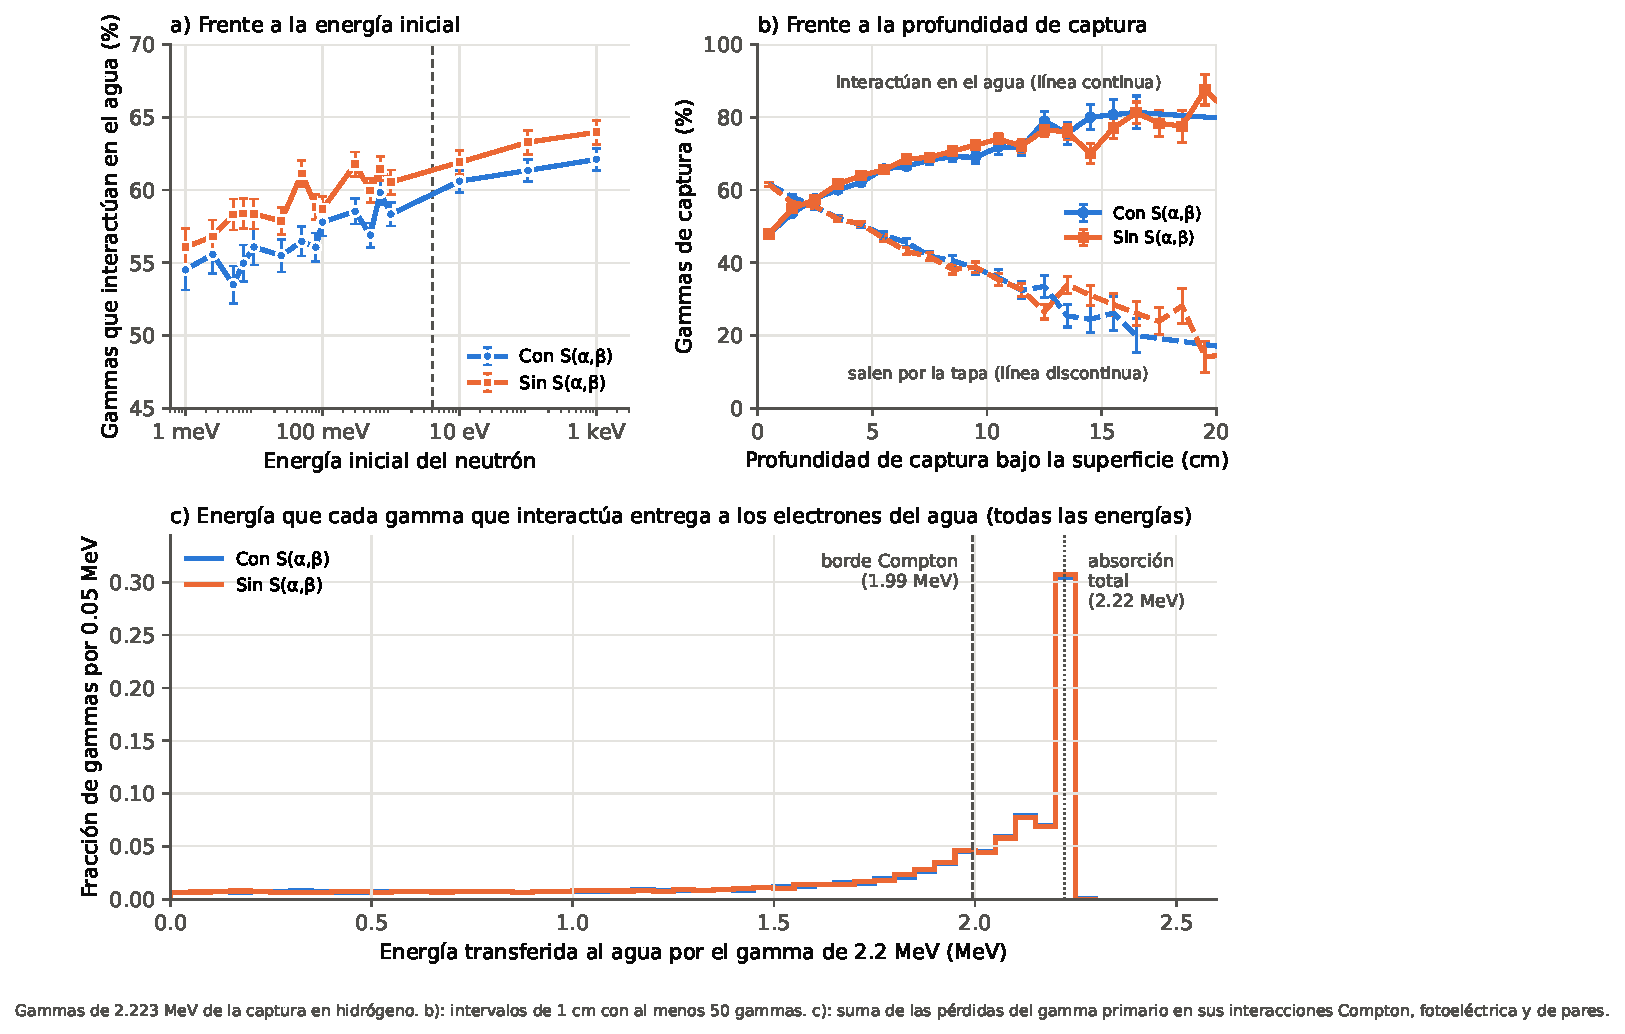
\includegraphics[width=\linewidth]{figuras/fig_contencion_gamma.pdf}
\caption{Fotones $\gamma$ de 2.223\,MeV de la captura en hidrógeno: fracción que interactúa en el agua (a) frente a la energía inicial del neutrón y (b) frente a la profundidad de captura, junto con la fracción que sale por la tapa; (c) energía que cada $\gamma$ que interactúa transfiere a los electrones del agua.}
\label{fig:contencion}
\end{figure}

\begin{itemize}
  \item \textbf{Solo entre el 54 y el 64\,\% de los $\gamma$ interactúan en el agua.} En conjunto, el 52\,\% sale por la tapa, el 26\,\% por la pared lateral, el 19\,\% se absorbe en el agua y el 4\,\% en la estructura. Es consecuencia directa de que las capturas ocurran a pocos centímetros de la superficie, mientras que un $\gamma$ de 2.2\,MeV necesita del orden de 20\,cm de agua para interactuar.
  \item \textbf{La contención depende solo de la profundidad de captura.} Un $\gamma$ emitido junto a la superficie interactúa en el 48\,\% de los casos y sale por la tapa en el 60\,\%; si se emite a 20\,cm, interactúa en el $\approx80$\,\%. Las curvas con y sin \sab{} coinciden (Figura~\ref{fig:contencion}b): la física electromagnética es la misma, y \sab{} influye únicamente al desplazar el punto de captura.
  \item \textbf{Energía transferida.} El espectro muestra el continuo Compton hasta el borde de 1.99\,MeV y un 31\,\% de absorciones totales (2.22\,MeV) tras varias interacciones, la forma esperada para un $\gamma$ de esta energía en agua.
\end{itemize}

\subsection{Procesos de interacción y origen de la luz}

\begin{figure}[H]
\centering
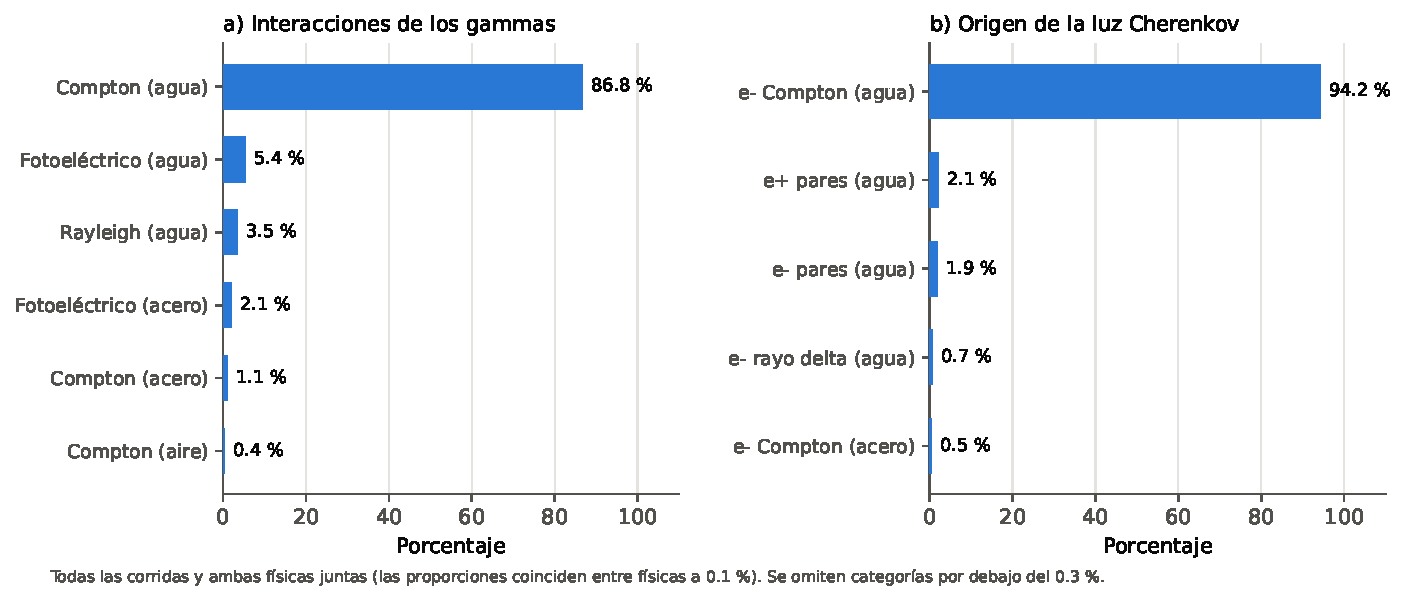
\includegraphics[width=\linewidth]{figuras/fig_procesos_luz.pdf}
\caption{(a) Interacciones de todos los fotones $\gamma$, por proceso y material. (b) Contribución de cada tipo de electrón o positrón a la luz Cherenkov total.}
\label{fig:procesos}
\end{figure}

El efecto Compton en el agua representa el 86.8\,\% de todas las interacciones de los $\gamma$, seguido del fotoeléctrico (5.4\,\%) y del Rayleigh (3.5\,\%) en el agua y del fotoeléctrico en el acero (2.1\,\%); la producción de pares es el 0.2\,\%. Las proporciones coinciden con y sin \sab{} a 0.1\,\%. Los electrones Compton del agua emiten el 94.2\,\% de la luz Cherenkov. Los pares $e^+e^-$ aportan el 4\,\%, pese a su escasa frecuencia, porque cada partícula sale con $\approx1.5$\,MeV. Los electrones fotoeléctricos, con energías de unos 20\,keV, no aportan luz.

\subsection{Electrones secundarios y umbral Cherenkov}

\begin{figure}[H]
\centering
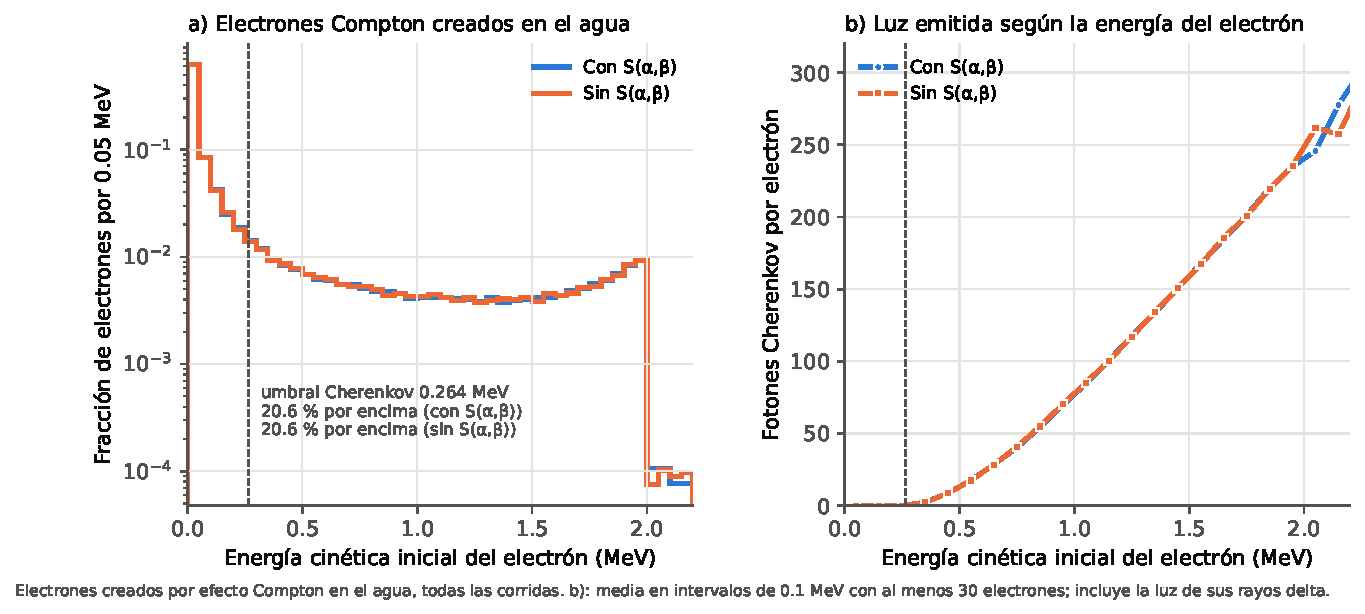
\includegraphics[width=\linewidth]{figuras/fig_electrones_cherenkov.pdf}
\caption{(a) Espectro de energía cinética inicial de los electrones Compton creados en el agua. (b) Número medio de fotones Cherenkov emitidos por electrón según su energía inicial.}
\label{fig:electrones}
\end{figure}

El espectro de los electrones Compton combina un pico intenso a baja energía, debido a los fotones ya degradados por dispersiones previas, con el borde Compton en 1.99\,MeV. \textbf{Solo el 20.6\,\% de ellos supera el umbral Cherenkov del agua} ($T_\mathrm{umbral}=m_e\left[(1-n^{-2})^{-1/2}-1\right]=0.264$\,MeV para $n=1.33$), con ambas físicas. La luz emitida es nula por debajo del umbral y crece con la energía: $\approx85$ fotones a 1\,MeV y $\approx240$ a 2\,MeV.

\subsection{De la luz a la carga}

\begin{figure}[H]
\centering
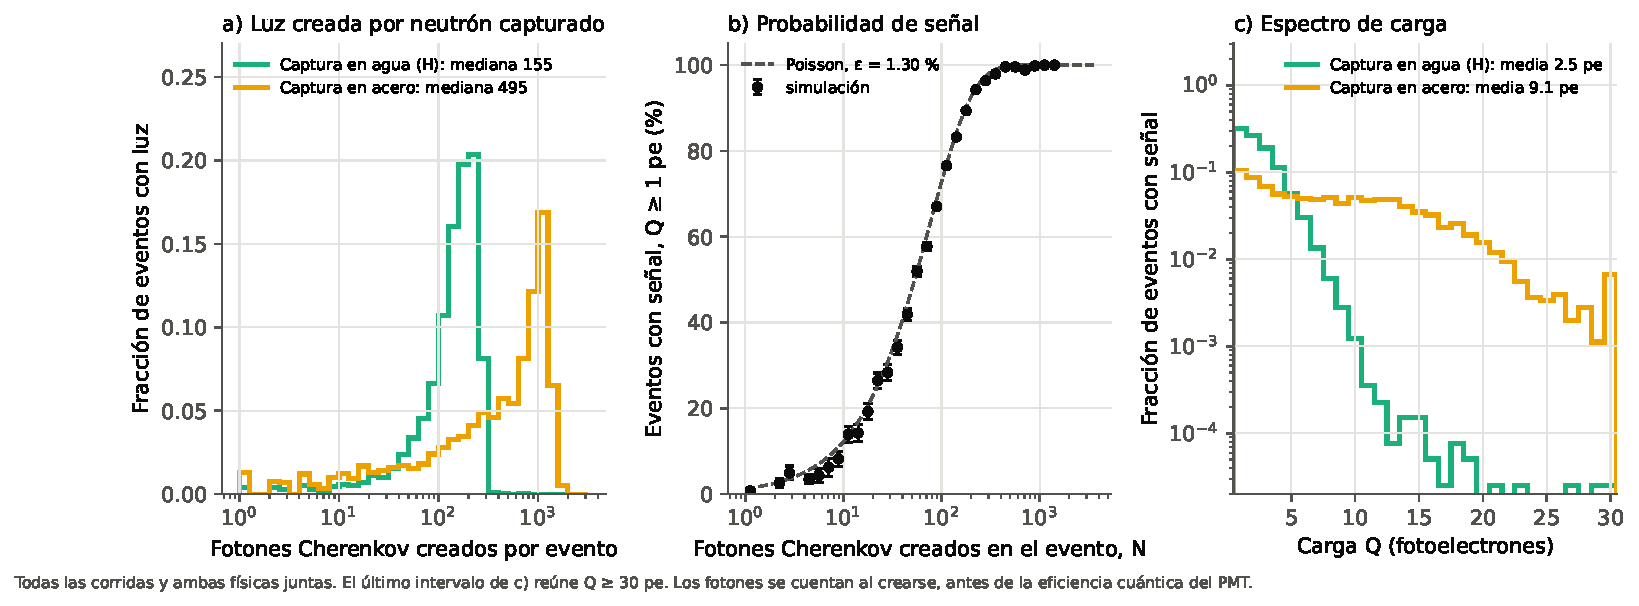
\includegraphics[width=\linewidth]{figuras/fig_luz_carga.pdf}
\caption{(a) Fotones Cherenkov creados por evento en capturas en el agua y en el acero. (b) Probabilidad de señal frente al número de fotones creados, comparada con un modelo de Poisson. (c) Espectro de carga de los eventos con señal.}
\label{fig:luzcarga}
\end{figure}

\begin{itemize}
  \item \textbf{Luz por captura.} Los eventos con luz crean una mediana de 155 fotones Cherenkov en una captura en hidrógeno y de 495 en una captura en el acero.
  \item \textbf{Solo el $1.30$\,\% de los fotones creados produce un fotoelectrón.} Este factor combina la geometría de colección, la absorción óptica y la eficiencia cuántica, y es el mismo con ambas físicas y para ambos orígenes. La probabilidad de señal sigue la estadística de Poisson, $P(Q\geq1)=1-\exp(-0.0130\,N)$: se necesitan $\approx53$ fotones para un 50\,\% de probabilidad y $\approx230$ para un 95\,\%.
  \item \textbf{Espectro de carga.} Las capturas en hidrógeno dan 2.5\,pe de media, con una caída rápida; las capturas en el acero dan 9.1\,pe, con una cola que supera los 30\,pe.
\end{itemize}

\subsection{La cadena completa}

\begin{table}[H]
\centering
\small
\begin{tabularx}{\linewidth}{>{\raggedright\arraybackslash}Xrrrr}
\toprule
& \multicolumn{2}{c}{25\,meV} & \multicolumn{2}{c}{1\,keV} \\
\cmidrule(lr){2-3}\cmidrule(lr){4-5}
Eslabón & con \sab{} & sin \sab{} & con \sab{} & sin \sab{} \\
\midrule
Neutrón capturado en el agua (\% de incidentes) & 19.7 & 28.3 & 41.9 & 33.5 \\
Su $\gamma$ interactúa en el agua (\% de capturas) & 55.5 & 57.9 & 62.2 & 64.0 \\
El evento produce luz Cherenkov (\% de capturas) & 53.2 & 55.5 & 59.2 & 61.1 \\
La luz produce $Q\geq1$ (\% de eventos con luz) & 75.8 & 78.5 & 77.7 & 76.9 \\
Señal tras la captura en el agua (\% de capturas) & 40.4 & 43.6 & 46.0 & 47.0 \\
\midrule
Detectados por captura en el agua (\% de incidentes) & 7.95 & 12.33 & 19.28 & 15.77 \\
Detectados en total, incluida la estructura (\% de incidentes) & 8.95 & 13.55 & 19.46 & 16.13 \\
\bottomrule
\end{tabularx}
\caption{Eslabones de la cadena de detección para dos energías iniciales.}
\label{tab:cadena}
\end{table}

\textbf{Los dos cuellos de botella del detector son geométricos}: el escape de los $\gamma$ por la tapa, consecuencia de la captura superficial, y la colección de solo el 1.3\,\% de los fotones Cherenkov. La física neutrónica, y con ella \sab{}, fija el primer eslabón; los siguientes dependen de ella solo a través de la profundidad de captura.

%------------------------------------------------
\section{Implicaciones para la tesis}
%------------------------------------------------

\begin{enumerate}
  \item \textbf{La diferencia entre campañas se debe a \sab{}.} Con geometría idéntica, el cociente de captura con y sin \sab{} a 25\,meV es 0.70 ($19.70/28.31$), prácticamente el 0.69 observado entre la Campaña~2 y la Campaña~1. La atribución previa de esa diferencia a la tapa de acero debe corregirse.
  \item \textbf{El máximo de captura entre 0.3 y 10\,eV es una propiedad del modelo de gas libre.} Con \sab{} la captura no presenta máximo: crece de forma monótona y se estabiliza en $\approx42$\,\%. Las conclusiones de los Capítulos~4 y~5 que describen ese máximo como efecto del albedo deben matizarse.
  \item \textbf{Región térmica.} Por debajo de 0.1\,eV, la física sin \sab{} sobrestima la captura en el agua entre un 18 y un 47\,\% relativo (máximo a 7\,meV).
  \item \textbf{Región epitérmica, la relevante para CRNS.} Entre 10\,eV y 1\,keV, \sab{} eleva la eficiencia de captura estimada del $\approx34$ al $\approx42$\,\%, un 21--25\,\% relativo más.
  \item \textbf{Diseño del detector.} Con incidencia desde la tapa, casi toda la captura y, por tanto, la emisión de la cascada $\gamma$ ocurren en los primeros $\sim$10\,cm bajo la superficie del agua. Este resultado es relevante para la posición del PMT y la colección de luz.
  \item \textbf{Física recomendada.} Para agua a temperatura ambiente, \sab{} es la descripción físicamente correcta del hidrógeno ligado; se recomienda usar QGSP\_BERT\_HP con \var{G4ThermalNeutrons} en las corridas definitivas.
  \item \textbf{Eficiencia de detección.} El observable del detector, la eficiencia $\varepsilon(E)$, reproduce el efecto de \sab{} sobre la captura, pero con el cruce en $\approx0.7$\,eV. La curva de eficiencia usada para la respuesta de referencia (Sección~4.6 de la tesis) debe recalcularse con \sab{}.
  \item \textbf{Pérdidas geométricas.} Con incidencia desde la tapa, casi la mitad de los $\gamma$ de captura escapa sin interactuar y solo el 1.3\,\% de la luz se convierte en fotoelectrones. Estas dos pérdidas, y no la física neutrónica, limitan la eficiencia; son los parámetros de diseño con más margen de mejora.
  \item \textbf{Papel del acero.} A energías térmicas y frías, las capturas en la tapa de acero aportan hasta un tercio de la señal, con cargas altas. Debe tenerse en cuenta al comparar con medidas y con tanques de otro material.
\end{enumerate}

%------------------------------------------------
\section{Limitaciones}
\label{sec:limitaciones}
%------------------------------------------------

\begin{itemize}
  \item \textbf{Estadística.} 10\,000 neutrones por punto: incertidumbre de $\approx0.5$ puntos en la captura; se observaron fluctuaciones de hasta 2.5$\sigma$ entre repeticiones. Suficiente para el panorama cualitativo, no para las cifras finales.
  \item \textbf{Solo agua pura.} El cloro de las soluciones con NaCl tiene una sección eficaz de captura unas 100 veces mayor que el hidrógeno y acortará aún más el camino térmico; el efecto de \sab{} puede cambiar con la salinidad. El material \var{SaltyWater} de MEIGA también usa hidrógeno ligado \var{TS\_H\_of\_Water}.
  \item \textbf{Incidencia vertical desde la tapa}, en un círculo de 40\,cm de radio y desde 67\,cm por encima de ella. Un campo de albedo real es aproximadamente isótropo e incide también por los lados.
  \item \textbf{Semilla aleatoria.} El simulador inicializa la semilla con \var{time(NULL)} y no la registra; las corridas no son reproducibles evento a evento, aunque sí estadísticamente.
  \item \textbf{Corte de producción.} El corte de 1\,mm ($\approx0.35$\,MeV para electrones en agua) impide crear rayos delta de menor energía; esto no afecta a la luz Cherenkov, porque esos electrones estarían casi todos bajo el umbral.
  \item \textbf{Energía transferida por los $\gamma$.} Se suma solo sobre el $\gamma$ de captura; no sigue a los $\gamma$ secundarios de aniquilación o bremsstrahlung.
  \item \textbf{Respuesta óptica.} La colección de luz (1.30\,\%) depende de las propiedades ópticas del modelo (absorción, reflectividad del Tyvek, eficiencia cuántica), cuyas incertidumbres no se propagaron.
  \item \textbf{Archivo excluido.} \archivo{pasos-particulas.tsv} (5.5\,GB) no se transfirió; se conserva en el contenedor. No es necesario para los análisis de este informe.
\end{itemize}

%------------------------------------------------
\section{Recomendaciones}
%------------------------------------------------

\begin{enumerate}
  \item Repetir el barrido con 100\,000 neutrones por punto para las cifras de la tesis (del orden de 25--30\,h de cómputo y 75\,GB comprimidos).
  \item Extender el barrido a las soluciones con 2.5, 5 y 10\,\% de NaCl.
  \item Estudiar configuraciones que aumenten la contención de los $\gamma$ y la colección de luz (posición del PMT, número de PMT, reflectividad del revestimiento), que son los factores que más limitan la eficiencia.
  \item Repetir el análisis electromagnético con NaCl: las cascadas del cloro ($\approx8.6$\,MeV en varios $\gamma$) deberían aumentar tanto la contención como la luz por captura.
  \item Estudiar incidencia isótropa o un espectro de albedo realista.
  \item Registrar la semilla aleatoria de cada corrida en el archivo de salida.
  \item Actualizar los Capítulos~4 y~5 con los resultados de \sab{}.
\end{enumerate}

%------------------------------------------------
\section{Reproducibilidad}
%------------------------------------------------

\begin{table}[H]
\centering
\small
\begin{tabularx}{\linewidth}{lX}
\toprule
Elemento & Ubicación \\
\midrule
Código del simulador & \archivo{wcd-nacl-crns-simulations}, rama \var{main}; etiquetas \var{campana-1-QGSP\_BERT\_HP} y \var{campana-2-QGSP\_BERT\_HP-SalphaBeta} \\
Kit de simulación & \archivo{simulations/barrido-SalphaBeta_1meV-1keV/} (\archivo{barrido.sh}, \archivo{correr_prueba.sh}, \archivo{resumen_prueba.sh}, \archivo{tabla_barrido.sh}) \\
Datos (7.5\,GB) & fuera del repositorio: \archivo{Prueba-agua-pura-1meV-1keV-dos-libreria/};\newline copia comprimida \archivo{barrido-1meV-1keV.tar.gz} (1.6\,GB) \\
Análisis e informe & \archivo{analysis/efecto-SalphaBeta_barrido-energia/} \\
\bottomrule
\end{tabularx}
\end{table}

Dentro del contenedor, el barrido completo se lanza con:
\begin{lstlisting}
cd /opt/Prueba-agua-pura-1meV-1keV-dos-libreria
./barrido.sh 0.001 0.0025 0.005 0.007 0.01 0.025 0.05 0.08 0.1 0.3 0.5 0.7 1 10 100 1000
\end{lstlisting}
y los análisis, las figuras y las tablas de este informe se regeneran con:
\begin{lstlisting}
cd analysis/efecto-SalphaBeta_barrido-energia
D=<carpeta de datos del barrido>
./balance_destinos.sh $D > balance_destinos.tsv
./capturas_detalle.sh $D > capturas_detalle.tsv
python3 figuras_barrido.py && python3 figuras_capturas.py
./em_detalle.sh $D
./em_cadena.sh $D
python3 figuras_em.py && python3 figuras_em2.py
cd informe && python3 generar_tablas.py && latexmk -pdf Informe-tecnico-Efecto-SalphaBeta-Barrido-Energia.tex
\end{lstlisting}

\appendix
\section{Destinos de los neutrones}
\label{app:destinos}

{\small\renewcommand{\arraystretch}{1.05}\begin{longtable}{llrrrrrr}
\caption{Destino de los neutrones incidentes, en porcentaje: captura en el agua, captura en la estructura (acero y Tyvek), reflexión por la tapa, escape lateral, transmisión por el fondo y desviación en el aire antes de llegar al tanque.}\\
\toprule
$E_0$ & Física & Agua & Estructura & Tapa & Lateral & Fondo & Aire \\
\midrule
\endfirsthead
\toprule
$E_0$ & Física & Agua & Estructura & Tapa & Lateral & Fondo & Aire \\
\midrule
\endhead
1\,meV & con $S(\alpha,\beta)$ & 12.95 & 8.96 & 72.38 & 0.07 & 0.00 & 5.64 \\
 & sin $S(\alpha,\beta)$ & 15.32 & 8.07 & 70.51 & 0.39 & 0.00 & 5.71 \\
\addlinespace[2pt]
2.5\,meV & con $S(\alpha,\beta)$ & 14.09 & 6.77 & 74.68 & 0.08 & 0.00 & 4.38 \\
 & sin $S(\alpha,\beta)$ & 18.47 & 5.88 & 71.13 & 0.33 & 0.00 & 4.19 \\
\addlinespace[2pt]
5\,meV & con $S(\alpha,\beta)$ & 15.16 & 5.47 & 75.89 & 0.12 & 0.00 & 3.36 \\
 & sin $S(\alpha,\beta)$ & 21.07 & 4.94 & 70.46 & 0.31 & 0.00 & 3.22 \\
\addlinespace[2pt]
7\,meV & con $S(\alpha,\beta)$ & 15.61 & 5.09 & 76.14 & 0.13 & 0.00 & 3.03 \\
 & sin $S(\alpha,\beta)$ & 22.90 & 4.67 & 68.81 & 0.36 & 0.00 & 3.26 \\
\addlinespace[2pt]
10\,meV & con $S(\alpha,\beta)$ & 16.14 & 4.08 & 76.71 & 0.16 & 0.00 & 2.91 \\
 & sin $S(\alpha,\beta)$ & 23.08 & 3.84 & 69.92 & 0.47 & 0.00 & 2.69 \\
\addlinespace[2pt]
25\,meV & con $S(\alpha,\beta)$ & 19.70 & 2.80 & 74.51 & 0.10 & 0.00 & 2.89 \\
 & sin $S(\alpha,\beta)$ & 28.31 & 2.94 & 65.80 & 0.40 & 0.00 & 2.55 \\
\addlinespace[2pt]
50\,meV & con $S(\alpha,\beta)$ & 23.64 & 2.43 & 71.26 & 0.21 & 0.00 & 2.46 \\
 & sin $S(\alpha,\beta)$ & 30.48 & 2.54 & 63.81 & 0.41 & 0.00 & 2.76 \\
\addlinespace[2pt]
80\,meV & con $S(\alpha,\beta)$ & 25.40 & 2.11 & 69.62 & 0.12 & 0.00 & 2.75 \\
 & sin $S(\alpha,\beta)$ & 32.07 & 2.20 & 62.60 & 0.52 & 0.00 & 2.61 \\
\addlinespace[2pt]
100\,meV & con $S(\alpha,\beta)$ & 26.32 & 1.99 & 69.02 & 0.13 & 0.00 & 2.54 \\
 & sin $S(\alpha,\beta)$ & 32.16 & 1.95 & 62.93 & 0.48 & 0.00 & 2.48 \\
\addlinespace[2pt]
300\,meV & con $S(\alpha,\beta)$ & 32.62 & 1.56 & 63.60 & 0.17 & 0.00 & 2.05 \\
 & sin $S(\alpha,\beta)$ & 33.00 & 1.87 & 62.12 & 0.64 & 0.00 & 2.37 \\
\addlinespace[2pt]
500\,meV & con $S(\alpha,\beta)$ & 35.39 & 1.39 & 60.72 & 0.19 & 0.00 & 2.31 \\
 & sin $S(\alpha,\beta)$ & 34.02 & 1.53 & 61.30 & 0.71 & 0.00 & 2.44 \\
\addlinespace[2pt]
700\,meV & con $S(\alpha,\beta)$ & 36.54 & 1.26 & 59.54 & 0.33 & 0.00 & 2.33 \\
 & sin $S(\alpha,\beta)$ & 34.20 & 1.83 & 61.10 & 0.56 & 0.01 & 2.30 \\
\addlinespace[2pt]
1\,eV & con $S(\alpha,\beta)$ & 37.76 & 0.96 & 58.61 & 0.25 & 0.00 & 2.42 \\
 & sin $S(\alpha,\beta)$ & 34.49 & 1.51 & 60.99 & 0.68 & 0.00 & 2.33 \\
\addlinespace[2pt]
10\,eV & con $S(\alpha,\beta)$ & 41.85 & 0.70 & 55.00 & 0.41 & 0.00 & 2.04 \\
 & sin $S(\alpha,\beta)$ & 34.48 & 1.06 & 61.64 & 0.71 & 0.00 & 2.11 \\
\addlinespace[2pt]
100\,eV & con $S(\alpha,\beta)$ & 42.03 & 0.63 & 54.75 & 0.27 & 0.00 & 2.32 \\
 & sin $S(\alpha,\beta)$ & 33.73 & 0.86 & 62.75 & 0.66 & 0.00 & 2.00 \\
\addlinespace[2pt]
1\,keV & con $S(\alpha,\beta)$ & 41.90 & 0.50 & 55.11 & 0.57 & 0.00 & 1.92 \\
 & sin $S(\alpha,\beta)$ & 33.54 & 0.80 & 62.45 & 1.09 & 0.00 & 2.12 \\
\bottomrule
\end{longtable}
}

\end{document}
